\chapter{Preliminaries}
\label{chapterlabel2}

\section{GAN}

GAN stands for Generative Adversarial Network\cite{goodfellowGenerativeAdversarialNetworks2014a}, it is a machine learning framework where two networks simultaneously compete and learns from each other in the form of a two-player, zero-sum game. The network consists of a generator $\mathcal{G}$ that tries to mimic the target and a discriminator $\mathcal{D}$ tries to distinguish between real and generated input. This training framework is commonly used in computer vision tasks to generate high-quality images.

Major challenges exist in training GAN, it can fail easily due to various reasons such as mode-collapse (see appendix \ref{app:ml:mode_col}), vanishing gradient (see appendix \ref{app:ml:van_grad}), non-convergence (see appendix \ref{app:ml:non_conv}), instability, inappropriate design (e.g. under/overpowered discriminator, use of loss and optimization algorithm, etc.). Therefore a number of variations are proposed to improve it, and they are commonly adopted in most models described in this paper.


\subsection{Wasserstein GANs}
Wasserstein GAN\cite{arjovskyWassersteinGAN2017} is a type of GAN proposed to improve the stability of training vanilla GAN. Compared to vanilla GAN, Wasserstein GAN provides a better gradient, which is helpful for getting rid of problems such as mode collapse and provides more meaningful training curves for debugging and hyper-parameter tuning.

\begin{figure}
    \centering
    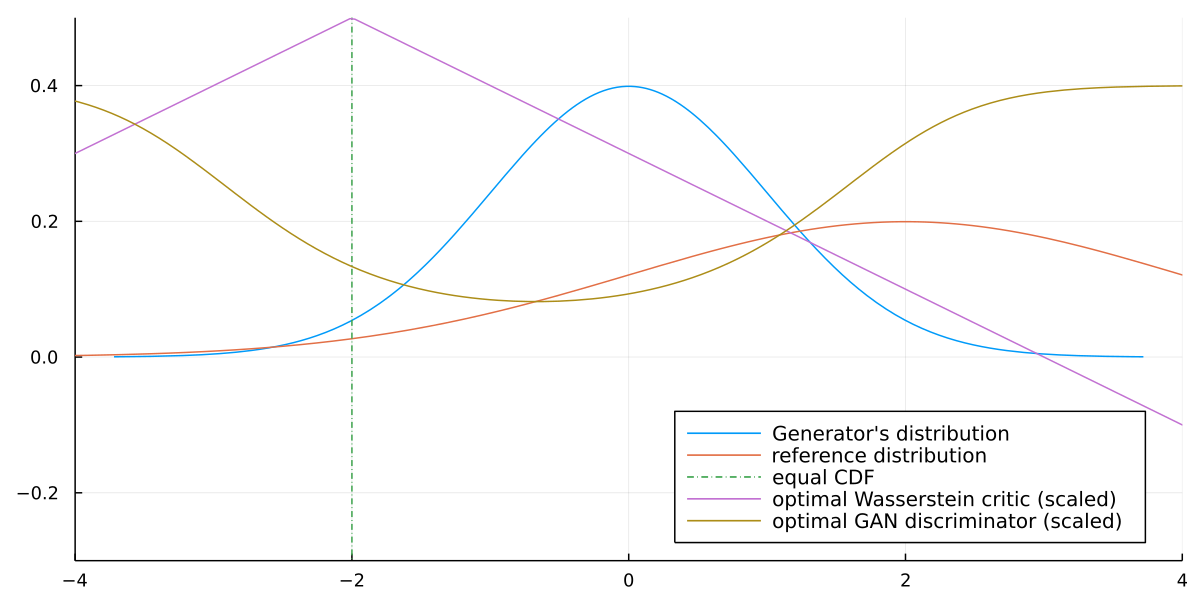
\includegraphics[width=0.75\textwidth]{images/preliminary/wgan_vs_gan_grad.png}
    \caption{Comparing the optimal Wasserstein function (scaled) and optimal GAN discriminator (scaled) given a fixed generator distribution and reference distribution. We can see that the gradient of the Wasserstein function is equal to $1$ for the optimal case, and gives less variance compared to the optimal GAN discriminator.\cite{FileWassersteinGANCritic}} 
    \label{fig:wgan_vs_gan_grad}
\end{figure}

Wasserstein GAN uses Wasserstein distance to compute the loss between actual and target distribution. It has the advantage of producing more consistent values when comparing distributions compared to other functions such as KL-divergence and JS-divergence. This means that its gradients have smaller variance and thus training is more stable (see figure \ref{fig:wgan_vs_gan_grad}). It is also practically useful because it is highly efficient to compute by satisfying the \textit{dual representation theorem} in metric space:

$$
W_{1}(\mu, \nu)=\frac{1}{K} \sup _{\|f\|_{L} \leq K} \mathbb{E}_{x \sim \mu}[f(x)]-\mathbb{E}_{y \sim \nu}[f(y)]
$$

where $W_1$ is the Wasserstein distance; $K$ is any fixed $K > 0$; $\sup$ means supremum (the largest, in other words, the upper bound); and $||\cdot||_L$ is the Lipschitz norm (Lipschitz constant with boundary condition)\footnote{A proof can be found at \url{https://en.wikipedia.org/wiki/Wasserstein\_metric\#Dual\_representation\_of\_W1}}. There are several methods for enforcing this constraint during training. The two most common methods are weight clipping (used in the original paper, see appendix \ref{app:ml:weight_clip}) and gradient penalty (see appendix \ref{app:ml:grad_pen}).

In practice, we would like our gradient to have a unit gradient norm almost everywhere. But by using weight clipping, the network will try to attain the maximum gradient and end up learning extremely simple functions\cite{gulrajaniImprovedTrainingWasserstein2017}. Additionally, it is hard to determine an appropriate clip value, because it involves many considerations such as model, dataset, and training procedure etc. By introducing the gradient penalty, instead of hard clipping the values, we are softly penalizing the model which is much more natural. Models that use gradient penalty to enforce bounded Lipschitz norms are called WGAN-GP.

\subsection{cGAN}
Conditional GAN (cGAN) is a type of GAN that have auxiliary information such as class labels or data from other sources as additional input. An ideal cGAN is able to produce a variety of outputs given different contextual information. Additionally, it also converges faster since additional information is provided.


\subsection{PatchGAN}
PatchGAN is a type of GAN that penalize the generator based on patches from the output image. Put simply, it is the use of the convolution layer as the first layer in the discriminator. Such discriminator models the image as Markov Random Field (MRF), assuming each pixel is only dependent on pixels near it.


\section{ResNet}
ResNet stands for Residual Neural Network. It is the first trainable network with hundreds of layers, by applying the residual/skip connection technique (see appendix \ref{app:ml:res_conn}). This technique was used extensively in succeeding networks.

\subsection{Pre-activation}
A number of residual connection variants were investigated. ResNet with full-pre-activation (or ResNetV2) was proposed to improve the ease of training and reduces overfitting \cite{heIdentityMappingsDeep2016a}. The full-pre-activation architecture for any weight layer $f$ is :


\begin{align}
    \hat{f}(x) &= x + PA(PA(x))\\
    PA(x) &= f(ReLU(BN(x)))
\end{align}


where $BN$ denotes batch normalization, $PA$ stands for pre-activation and $\hat{f}(x)$ is the full-pre-activation function. 

%A more detailed analysis can be found at appendix \ref{app:ml:pre_act}.

\subsection{ResNeXt}
ResNeXt is a name given to Aggregated Residual Transformations\cite{xieAggregatedResidualTransformations2017a}. The ResNeXt block consists of $N$ smaller, parallel blocks that the input will go through, and $N$ outputs are summed to produce the final output. Formally, it can be represented as:

$$
f(x)=\sum^{C}_{i=1} \mathcal{T}_i(x)
$$

where $\mathcal{T}_i$ can be an arbitrary function, and $C$ is the \textit{cardinality} (the number of parallel paths). Figure \ref{fig:resnet_resnext_cmp} showed a more straight forward explanation. The paper suggests that when attempts to increase the capability of a ResNet network, instead of adding more layers, it is more \textit{cost} effective to increase the cardinality of the ResNet block. This means the model has a higher capability per parameter/computation ratio. i.e. with the same number of parameters, ResNeXt outperforms the corresponding ResNet architecture in various vision tasks.

\begin{figure}
    \centering
    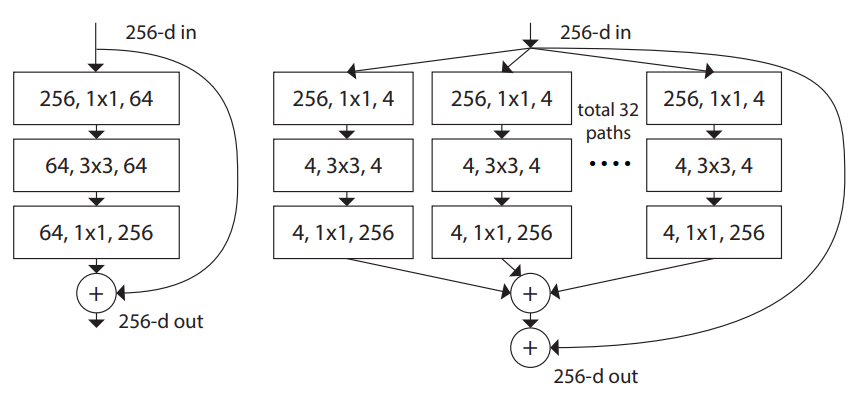
\includegraphics[width=0.75\textwidth]{images/preliminary/resnet_resnext_cmp.png}
    \caption{Comparison of ResNet and ResNeXt architecture. The left showed a typical block of ResNet and the right showed the corresponding ResNeXt architecture with cardinality \= 32. Both have roughly the same computational complexity. The numbers in the box correspond to \# input channels, filter size, and \# output channels.\cite{xieAggregatedResidualTransformations2017a}} 
    \label{fig:resnet_resnext_cmp}
\end{figure}

There are also other well-known variants of ResNet such as WideResNet and DenseNet. However, I will not introduce them because papers I read while researching dominantly chose to use ResNeXt architecture.



\section{Pix2pix}
Pix2pix is a cGAN-based image-to-image translation architecture. The architecture uses U-Net based generator and PatchGAN discriminator that penalizes the model on patches. It is not application-specific and can be applied to a wide range of vision tasks and yield reasonable results. These tasks include synthesizing photos from label maps, colourizing grayscale images, and converting sketches to photos.

\subsection{U-Net}
U-Net\cite{ronnebergerUNetConvolutionalNetworks2015} is commonly refers as a U-shaped encoder-decoder residual network architecture. It is originally developed for image segmentation in biomedical image processing (see figure \ref{fig:unet_arch}) based on a previous fully convolutional network study\cite{longFullyConvolutionalNetworks2015}. It is a popular approach in many vision tasks.

\begin{figure}
    \centering
    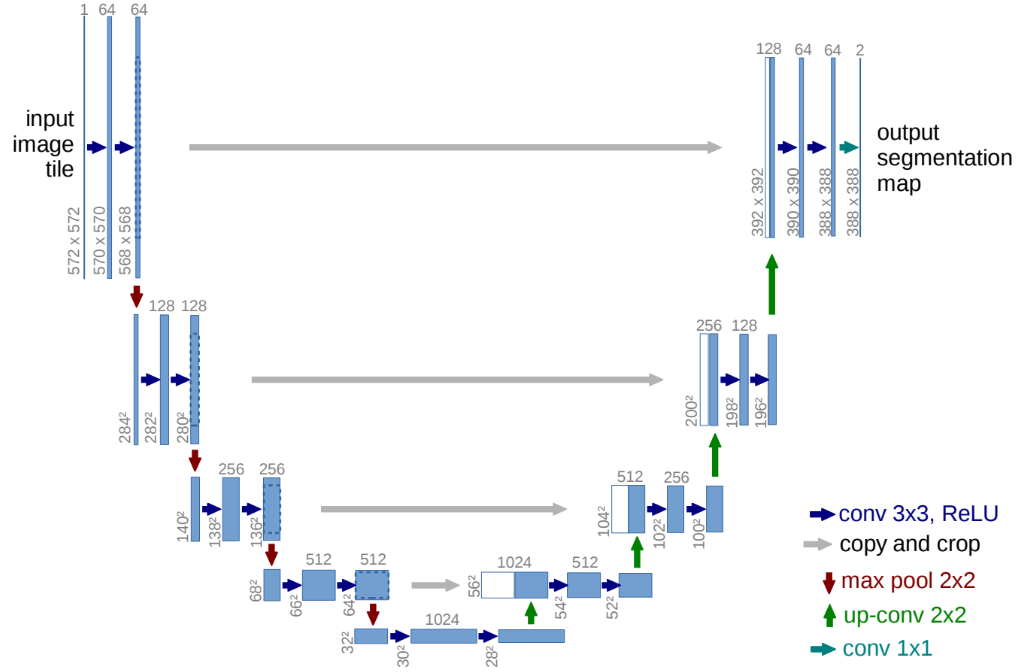
\includegraphics[width=0.75\textwidth]{images/preliminary/unet_arch.png}
    \caption{U-Net architecture. Light blue box corresponds to multi-channels features; the blue arrow is 3x3 convolution with ReLU; the grey arrow is copy and crop operations, more commonly known as skip/residual connection; the red arrow is 2x2 max pooling; the green arrow is 2x2 up convolution or interpolation, and the light blue arrow is 1x1 convolution for feature reduction.\cite{ronnebergerUNetConvolutionalNetworks2015}} 
    \label{fig:unet_arch}
\end{figure}

The first half of the network consists of a number of encoder blocks. Each consists of a convolutional block followed by a ReLU activation and max pooling. Each block halves the size of the feature map. The second half is similar to the first half, except it doubles the size of the feature map at each decoded block. The output of the corresponding encoder block is given as additional input to the decoder network, this operation is known as skip/residual connection.

Some implementations add a batch normalization between the convolution layer and the ReLU layer, in an attempt to reduce internal covariance shift and improve training stability. A dropout layer may also be added after ReLU as a form of regularization to improve the generalization of the network.
